% The Earth's orbit around the Sun
% Author: Julien Cretel, 25/02/2013
\documentclass{beamer}
\usepackage{tikz}
\setbeamertemplate{navigation symbols}{}

\begin{document}
\begin{frame}[fragile]
\frametitle{}
\begin{center}
  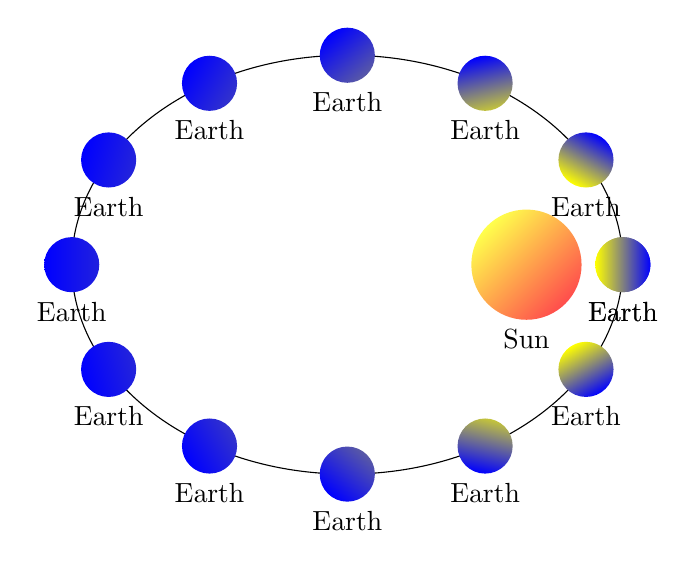
\begin{tikzpicture}[scale=3.5]
  \setbeamercovered{invisible}
  \pgfmathsetmacro{\Sunradius}{0.2}   % Sun radius
  \pgfmathsetmacro{\Earthradius}{0.1} % Earth radius
  \pgfmathsetmacro{\e}{0.65}          % Excentricity of the elliptical orbit
  \pgfmathsetmacro{\b}{sqrt(1-\e*\e)} % Minor radius (major radius = 1)

  % Draw the Sun at the right-hand-side focus
  \shade[
    top color=yellow!70,
    bottom color=red!70,
    shading angle={45},
   ] ({sqrt(1-\b*\b)},0) circle (\Sunradius);
  \visible<1>{
    \draw ({sqrt(1-\b*\b)},-\Sunradius) node[below] {Sun};
  }

  % Draw the elliptical path of the Earth.
  \draw[thin] (0,0) ellipse (1 and {\b});
  	
  % This function computes the direction in which light hits the Earth.
  \pgfmathdeclarefunction{f}{1}{%
    \pgfmathparse{
      ((-\e+cos(#1))<0) * ( 180 + atan( \b*sin(#1)/(-\e+cos(#1)) ) ) 
        +
      ((-\e+cos(#1))>=0) * ( atan( \b*sin(#1)/(-\e+cos(#1)) ) ) 
    }
  }

  % This function computes the distance between Earth and the Sun,
  % which is used to calculate the varying radiation intensity on Earth.
  \pgfmathdeclarefunction{d}{1}{%
    \pgfmathparse{ sqrt((-\e+cos(#1))*(-\e+cos(#1))+\b*sin(#1)*\b*sin(#1)) }
  }
						
  % Produces a series of frames showing one revolution
  % (the total number of frames is controlled by macro \N)
  \pgfmathtruncatemacro{\N}{12}
  \foreach \k in {0,1,...,\N}{
    \pgfmathsetmacro{\theta}{360*\k/\N}
      \pgfmathsetmacro{\radiation}{100*(1-\e)/(d(\theta)*d(\theta))}
      \colorlet{Earthlight}{yellow!\radiation!blue}
      \pgfmathparse{int(\k+1)}
      \onslide<\pgfmathresult>{
        % \onslide is used instead of \visible<.-(x)> and \pause,
        % in order not to break header and footer.
        \shade[
          top color=Earthlight,
          bottom color=blue,
          shading angle={90+f(\theta)},
        ] ({cos(\theta)},{\b*sin(\theta)}) circle (\Earthradius);
        \visible<1>{
          \draw ({cos(\theta)},{\b*sin(\theta)-\Earthradius}) node[below] {Earth};		
        }
      }
    }
  \end{tikzpicture}
\end{center}
\end{frame}
\end{document}